\documentclass[a4paper,10pt]{report}
\usepackage[utf8]{inputenc}
\usepackage[francais]{babel}
\usepackage[top=1.5cm, bottom=1.5cm, left=1cm, right=1cm]{geometry}
\usepackage{graphicx}

% Title Page
\title{OMGL4 - Etape 3 : expression des besoins, analyse et conception des autres cas d'utilisation}
\author{MAILLET Arnaud (chef de projet), VARGAS Christophe, ARDAUD Guillaume}


\begin{document}
\maketitle
\newpage
\null
\newpage
\tableofcontents
\newpage
\null
\newpage

\centering

\chapter*{Nouveau numéro périodique}
\addcontentsline{toc}{chapter}{Nouveau numéro périodique}
\section*{Diagramme de séquence haut niveau}
\addcontentsline{toc}{section}{Diagramme de séquence haut niveau}

Auteur : Arnaud MAILLET
Relecteur : xx

\bigskip

\begin{flushleft}
- La documentaliste demande l'enregistrement pour un nouveau numéro d'un périodique donné.\\
- Le système demande le numéro ISSN du périodique.\\
- La documentaliste saisit le numéro ISSN du périodique.\\
- Le système recherche le périodique dans le système informatique et affiches ses informations propres (nom périodique).\\
- Le système demande le numéro de parution du nouveau numéro du périodique.\\
- La documentaliste saisit le numéro de parution du nouveau numéro du périodique.\\
- Le système créé le numéro du périodique et affecte le numéro au periodique.\\
- Le système demande les informations propres des articles du numéro du periodique (titre, page, auteur(s), mot(s) clé(s)).\\
- La documentaliste saisit les informations propres des articles du numéro du périodique.\\
- Le système confirme l'enregistrement du nouveau numéro du periodique.\\
\end{flushleft}

\bigskip

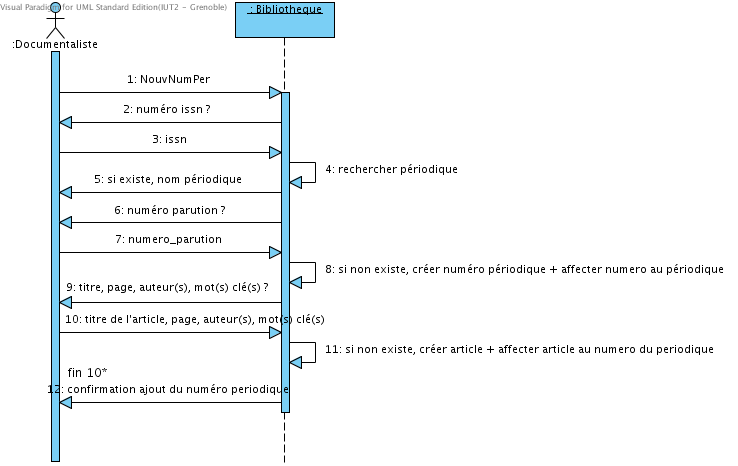
\includegraphics[height=115mm]{NouvNumPerHautNiveau.png}

\newpage

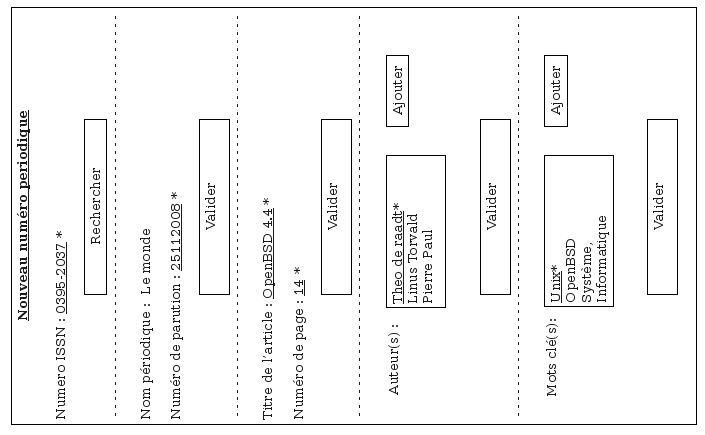
\includegraphics[height=100mm]{UpNouvNumPer.png}


\end{document}
